\subsection{UC30 - Eliminazione suddivisione}
\begin{figure}[H]
  \centering
  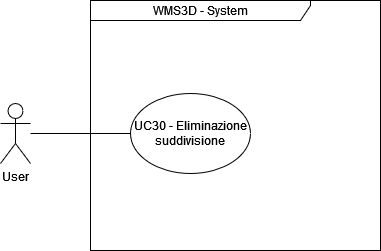
\includegraphics[width=0.5\textwidth]{UC_diagrams_28-32/UC30_sys.drawio.png}
  \caption{Diagramma UML UC30 - Eliminazione suddivisione}
\end{figure}
\begin{itemize}
    \item \textbf{Attori:} User.
    \item \textbf{Pre-condizione:} L'utente ha selezionato una suddivisione del magazzino precedentemente creata [UC28] da eliminare.
    \item \textbf{Post-condizione:} Lo spazio della suddivisione non è più adibito a nessuno scopo specifico, posso dunque creare altre suddivisioni al suo posto.
    \item \textbf{Scenario Principale:} L'utente seleziona una suddivisione e la elimina.
    \item \textbf{Generalizzazioni:} -
    \item \textbf{Estensioni:} -
\end{itemize}